\chapter{Modellistica ed equazioni differenziali lineari}

\section{Circuiti elettrici}

\begin{center}
  \begin{tabular}{|l l|}
  \hline
    Resistenza & $v(t) = Ri(t)$ \\
    Induttanza & $v(t) = L\frac{di(t)}{dt} = LDi$ \\
    Capacità & $v(t) = \frac{1}{C}\int_{-\infty}^t i(\tau) \rightarrow Dv_C = \frac{i}{C}$ \\
  \hline
  \end{tabular}
\end{center}

\section{Sistema meccanico}
\begin{center}
  \begin{tabular}{|l l|}
  \hline
    Massa & $MD^2x(t) = f_1(t)-f_2(t)$ \\
    Molla & $f(t) = K(x_1(t) - x_2(t))$ \\
    Ammortizzatore & $f(t) = BD(x_1(t) - x_2(t))$ \\
    \hline
  \end{tabular}
\end{center}



\section{OPAMP}
\begin{figure}[h!]
\centering
  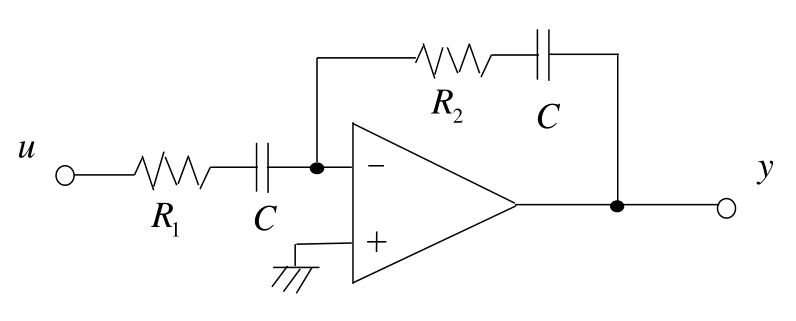
\includegraphics[width=0.4\linewidth]{images/opamp.png}
\end{figure}
Avendo $u$ tensione in ingresso e $y$ tensione in uscita, si ha che:
\begin{align}
  R_1CD_y + y = -R_2CDu - u
\end{align}


\section{Equazioni differenziali lineari}
Generalmente si ha che:

\begin{align}
  \sum_{i=0}^n a_iD^iy = \sum_{i=0}^m b_iD^iu
\end{align}

Dove:
\begin{itemize}
  \item $\rho = |n - m|$ ordine relativo o grado relativo
  \item $y$ è l'uscita
  \item $u$ è l'ingresso
\end{itemize}
